\documentclass[letterpaper]{article}
\usepackage[utf8]{inputenc}
\usepackage[spanish, mexico]{babel}
\usepackage{amssymb, amsmath}
\usepackage{graphicx}
\usepackage[margin=1.5cm,
vmargin={1.5cm,0.7cm},
includefoot]{geometry}
\usepackage{amsthm}
\usepackage{dsfont}
\usepackage{mathtools}
\usepackage{graphicx}


\begin{document}
	
	\setlength{\unitlength}{1cm}
	\thispagestyle{empty}
	\begin{picture}(19,3)
		\put(-0.5,1.2){
\includegraphics[scale=.20]{img/unam1.png}}
		\put(16,1){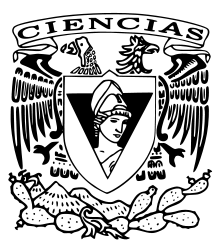
\includegraphics[scale=.29]{img/fciencias1.png}}
	\end{picture}
	
	\begin{center}
		\vspace{-114pt}
		\textbf{\large Computación concurrente}\\
		\textbf{ Semestre 2024-1}\\
		Prof. Gilde Valeria Rodríguez Jiménez\\
		Ayud. Luis Angel Leyva Castillo, Gibrán Aguilar Zuñiga, y Rogelio Alcantar Arenas  \\
		\textbf{Práctica 02}\\[0.08cm]
		Kevin Ariel Merino Peña\footnote{Número de cuenta 317031326} Roberto Adrián Bonilla Ruiz\footnote{Número de cuenta 317058163} Melissa Vázquez González\footnote{Número de cuenta 317209468}\\ [0.12cm]
		\today
	\end{center}
	\vspace{-5pt}
	\rule{19cm}{0.3mm}
	

	
	% -----------------------------------------------------
	% Así funcionan los comentarios aquí
	% -----------------------------------------------------
	
	
	
	\section{Implementación del algoritmo del filtro modificado}
		\subsection{Cumple mutual exclusion}
		\subsection{Cumple DeadLock-\textit{free}}
		\subsection{Cumple Starvation-free}
	\section{Solución del problema de los inversores}
		\subsection{Usando el candado cumple justicia}
		\subsection{Usando el filtro modificado cumple justicia}
	\section{Solución del problema del estacionamiento}
		\subsection{Cumple mutual exclusion}
		\subsection{Cumple DeadLock-\textit{free}}
		\subsection{Cumple Starvation-free}
		\subsection{Cumple Fairness}
	\section[APA]{Referencias}

	
	
\end{document}